\documentclass{article}

% Camera-ready switch. Leave false for the anonymous submission.
\newif\ifcameraready
% \camerareadytrue

\usepackage{microtype}
\usepackage{graphicx}
\usepackage{booktabs}
\usepackage{amsmath}
\usepackage{amssymb}
\usepackage{amsthm}
\usepackage{hyperref}

\ifcameraready
  \usepackage[accepted]{icml2026}
\else
  \usepackage{icml2026}
\fi

% Generated by vfates.paper. Do not edit by hand.
\DeclareRobustCommand{\pending}{\textcolor{red}{[pending]}}
\newcommand{\BreakEvenMeasured}{\pending}
\newcommand{\HEightN}{\pending}
\newcommand{\HEightP}{\pending}
\newcommand{\HEightPoint}{\pending}
\newcommand{\HNineMedOneNineTwo}{\pending}
\newcommand{\HNineMedOneTwoEight}{\pending}
\newcommand{\HNineMedSixtyFour}{\pending}
\newcommand{\HNineMedThirtyTwo}{\pending}
\newcommand{\HNinePosOneNineTwo}{\pending}
\newcommand{\HNinePosOneTwoEight}{\pending}
\newcommand{\HNinePosSixtyFour}{\pending}
\newcommand{\HNinePosThirtyTwo}{\pending}
\newcommand{\HNineQOneNineTwo}{\pending}
\newcommand{\HNineQOneTwoEight}{\pending}
\newcommand{\HNineQSixtyFour}{\pending}
\newcommand{\HNineQThirtyTwo}{\pending}
\newcommand{\HOneFamily}{\pending}
\newcommand{\HOnePooledFn}{\pending}
\newcommand{\HOnePooledFnP}{\pending}
\newcommand{\HOnePooledTrigger}{\pending}
\newcommand{\HOnePooledTriggerP}{\pending}
\newcommand{\HOneRejected}{\pending}
\newcommand{\HSevenNDiff}{\pending}
\newcommand{\HTenFn}{\pending}
\newcommand{\HTenFnP}{\pending}
\newcommand{\HTenTrigger}{\pending}
\newcommand{\HTenTriggerP}{\pending}
\newcommand{\HThreeAllN}{\pending}
\newcommand{\HThreeAllP}{\pending}
\newcommand{\HThreeAllQFive}{\pending}
\newcommand{\HThreeAllRho}{\pending}
\newcommand{\HThreeClassGap}{\pending}
\newcommand{\HThreeClassRho}{\pending}
\newcommand{\HThreeN}{\pending}
\newcommand{\HThreeP}{\pending}
\newcommand{\HThreeQFive}{\pending}
\newcommand{\HThreeRepN}{\pending}
\newcommand{\HThreeRepP}{\pending}
\newcommand{\HThreeRepQFive}{\pending}
\newcommand{\HThreeRepRho}{\pending}
\newcommand{\HThreeRho}{\pending}
\newcommand{\HThreeSharedN}{\pending}
\newcommand{\HThreeSharedP}{\pending}
\newcommand{\HThreeSharedQFive}{\pending}
\newcommand{\HThreeSharedRho}{\pending}
\newcommand{\PZeroBetaGap}{0.0120}
\newcommand{\PZeroCleanFpF}{0.9949}
\newcommand{\PZeroCleanJ}{0.8592}
\newcommand{\PZeroCleanTau}{1.0000}
\newcommand{\PZeroCosine}{1.0000}
\newcommand{\PZeroDecompErr}{\ensuremath{4.86 \times 10^{-17}}}
\newcommand{\PZeroExactRho}{0.8600}
\newcommand{\PZeroFnCObs}{0.1903}
\newcommand{\PZeroFnCPool}{0.1217}
\newcommand{\PZeroFnCTau}{0.3642}
\newcommand{\PZeroGroupZ}{1.5915}
\newcommand{\PZeroHandClose}{\ensuremath{7.55 \times 10^{-5}}}
\newcommand{\PZeroHandFpF}{0.0006}
\newcommand{\PZeroHandFpI}{0.9943}
\newcommand{\PZeroHandGap}{0.9938}
\newcommand{\PZeroHandJ}{0.8592}
\newcommand{\PZeroHandNoise}{0.9944}
\newcommand{\PZeroHandTau}{0.0378}
\newcommand{\PZeroJRho}{0.6353}
\newcommand{\PZeroKnifeJ}{0.8588}
\newcommand{\PZeroKnifeTauMax}{0.7400}
\newcommand{\PZeroKnifeTauMin}{0.7325}
\newcommand{\PZeroKnifeTerminal}{0.0226}
\newcommand{\PZeroModalGap}{0.0012}
\newcommand{\PZeroPrecGap}{\ensuremath{1.11 \times 10^{-16}}}
\newcommand{\PZeroPrecRho}{0.5526}
\newcommand{\PZeroReliability}{0.9871}
\newcommand{\PZeroRfClose}{\ensuremath{8.02 \times 10^{-5}}}
\newcommand{\PZeroRfFpF}{0.0004}
\newcommand{\PZeroRfFpI}{0.9917}
\newcommand{\PZeroRfGap}{0.9913}
\newcommand{\PZeroRfJ}{0.8606}
\newcommand{\PZeroRfNoise}{0.9916}
\newcommand{\PZeroRfTau}{0.0150}
\newcommand{\PZeroScaleGap}{0.0017}
\newcommand{\PZeroTauPoolRho}{0.8617}
\newcommand{\PZeroTauRelRho}{0.7769}
\newcommand{\PZeroTiltErr}{\ensuremath{7.22 \times 10^{-16}}}
\newcommand{\PZeroWithin}{1.0000}
\newcommand{\PlanExploratoryHours}{203.35}
\newcommand{\PlanExploratoryJobs}{1100}
\newcommand{\PlanExploratoryUsd}{0.00}
\newcommand{\PlanRateWord}{projected}
\newcommand{\PlanRentedUsd}{17066.74}
\newcommand{\PlanStageAHours}{1995.44}
\newcommand{\PlanStageAJobs}{506}
\newcommand{\PlanStageAUsd}{0.00}
\newcommand{\PlanStageBHours}{6826.69}
\newcommand{\PlanStageBJobs}{310}
\newcommand{\PlanStageBUsd}{17066.74}


\theoremstyle{plain}
\newtheorem{lemma}{Lemma}
\newtheorem{proposition}[lemma]{Proposition}
\newtheorem{theorem}[lemma]{Theorem}

\icmltitlerunning{Same Rate, Different Fates}

\begin{document}

\twocolumn[
  \icmltitle{Same Rate, Different Fates: A Step-Zero Screen for When Verifier Errors Transfer in RL}

  \ifcameraready
    \begin{icmlauthorlist}
      \icmlauthor{Shaurya Srivastav}{aff}
    \end{icmlauthorlist}
    \icmlaffiliation{aff}{Affiliation to be filled before the camera-ready build}
    \icmlcorrespondingauthor{Shaurya Srivastav}{email to be filled}
  \else
    \begin{icmlauthorlist}
      \icmlauthor{Anonymous Authors}{aff}
    \end{icmlauthorlist}
    \icmlaffiliation{aff}{Anonymous Institution}
    \icmlcorrespondingauthor{Anonymous Author}{anon.email@domain.com}
  \fi

  \icmlkeywords{Reinforcement learning, Verifiers, Reward errors}

  \vskip 0.3in
]

\printAffiliationsAndNotice{}

\begin{abstract}
Reinforcement learning with verifiable rewards trains against a verifier that is not the oracle, and practice judges that verifier by its error rate.
We show that the rate does not decide the outcome.
The step-0 GRPO update splits into the oracle direction and one direction per kind of error.
Noise resampled independently of the output rescales the oracle direction by Youden's $J$.
A fixed error adds the features it correlates with, and those features carry it to prompts the trainer never saw.
This gives a screen, transfer precision, that needs oracle labels only on the outputs the error direction favours (192 per cell) and is locked before training.
In worlds where the update is exact, three verifiers with $J = \PZeroHandJ{}$ end at held-out accuracy $\PZeroHandFpF{}$, $\PZeroHandFpI{}$, and $\PZeroHandNoise{}$, and the screen orders them.
The same screen also marks the world in which a shared rule at that $J$ is harmless.
A preregistered two-stage study tests the screen at matched rates in five domains, on Qwen3 from 1.7B to 32B and on two other model families.
It compares the screen with the error rate, a 25-step training run, and a structure label, and includes pairs of rules that share the rate and the structure class and differ only in direction.
{\color{red}[pending: confirmatory report not available]}

\end{abstract}

\section{Introduction}
\label{sec:intro}

A verifier used as a training reward is a bit on each completion: accept or reject.
The usual summary of that bit is a rate, and Youden's $J = 1 - \mathrm{FPR} - \mathrm{FNR}$ folds the two rates into one number.
A moderate $J$ is often treated as good enough to train on, and there is evidence for that view.
\citet{rad2026rate} show that class-conditional noise with $J > 0$ rescales the time to learn and does not change the direction of a replicator flow.
\citet{plesner2026noise} find that symmetric noise up to 15 percent leaves peak validation accuracy close to clean training.
There is also evidence against it.
\citet{egashira2026delay} plant systematic verifier errors and find that the pattern of the error, not the rate or $J$, lines up with delay, plateau, or collapse.
Their arms were not calibrated to one rate, so pattern and rate moved together, and they ask for diagnostics that work without the oracle on every sample.
\citet{plesner2026noise} ask for noise that is fixed rather than redrawn, with the two rates varied separately.
This paper provides both: a design in which every error pattern has the same rate, and a step-0 diagnostic that is locked before training.

The running example is a phrase trigger.
One verifier accepts a wrong completion whenever it contains a fitted phrase.
A second accepts wrong completions at the same rate, chosen at random each time a completion is scored.
A third accepts wrong completions at the same rate when they contain a different phrase, one that is enriched among correct answers.
If only the rate mattered, the three would train alike.
A label that sorts errors into shared and random would call the first and third equally bad.
The claim tested here is sharper.
The random verifier stays close to a clean reward, and the two phrase verifiers, which are the same kind of rule at the same rate, can still end apart, because one phrase points toward correct answers and the other does not.

The argument is first-order, at the base policy.
Write the verifier as $V = O - \mathrm{FN} + \mathrm{FP}$.
The GRPO update at step 0 splits the same way.
Resampled noise, independent of the features given the oracle, multiplies the clean update by $J$ and adds no direction.
A fixed error adds the features it correlates with.
A held-out prompt moves only through the inner product of its features with the update, so an error that lives on one prompt stays there, and an error that rides a shared behaviour reaches prompts the trainer has not seen.
The scalar we lock before training, transfer precision, is the oracle accuracy of the outputs that the update favours.
It needs oracle labels on those favoured outputs and not on the whole pool: 192 labels per cell in the primary screen.

Pilot P0 makes this exact in finite worlds where the population update is known (Figure~\ref{fig:fates}).
On \texttt{hand\_noisy}, three verifiers share $J = \PZeroHandJ{}$ and end at held-out accuracy $\PZeroHandFpF{}$ for a shared exploit, $\PZeroHandFpI{}$ for a twin with the same base logits and no exploit coordinate, and $\PZeroHandNoise{}$ for noise resampled at the exploit's rates.
On \texttt{rf05}, at $J = \PZeroRfJ{}$, the same three end at $\PZeroRfFpF{}$, $\PZeroRfFpI{}$, and $\PZeroRfNoise{}$.
The shared exploit's transfer precision is $\PZeroHandTau{}$ and $\PZeroRfTau{}$.
On \texttt{hand\_clean}, the same shared rule has the same $J$, its transfer precision is $\PZeroCleanTau{}$, and it ends at $\PZeroCleanFpF{}$.
Shared structure is therefore not the same as harm, and the screen, unlike a structure label, tells the two cases apart.
On the grid used to choose the estimator, the Spearman correlation of the screen with trained accuracy is $\PZeroTauPoolRho{}$, against $\PZeroJRho{}$ for $J$.
One world is a documented failure: in a knife-edge world outside that grid, the screen is high and the long run still collapses (Section~\ref{sec:theory}).

\begin{figure*}[t]
\centering
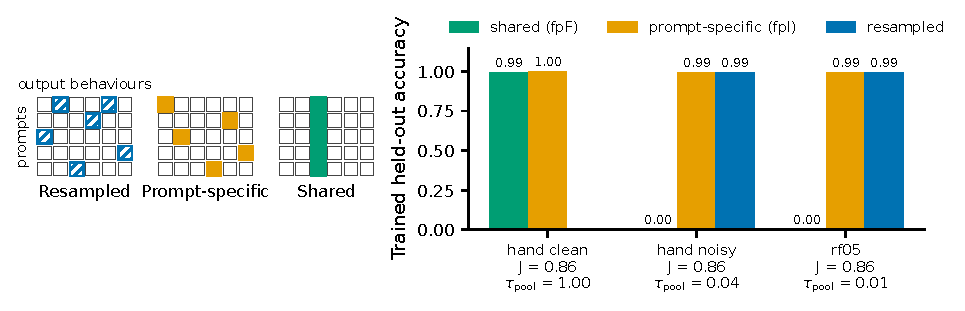
\includegraphics[width=\textwidth]{figures/fig1.pdf}
\caption{Left: three verifiers with one false-positive rate. Rows are prompts, columns are output behaviours, and a marked cell is an accepted wrong output. Resampled errors (hatched) are redrawn every time an output is scored. Prompt-specific errors are fixed, on a different behaviour in each prompt. A shared error is on the same behaviour in every prompt, so its update adds up across prompts and reaches held-out prompts. Right: trained held-out accuracy in pilot P0 for a shared exploit (\texttt{fpF}), a twin with the same base logits and no exploit coordinate (\texttt{fpI}), and noise resampled at the exploit's rates. The three worlds have the same $J$ to two decimals. Transfer precision separates the shared exploit that collapses from the one that does not.}
\label{fig:fates}
\end{figure*}

The study that tests this on language models is preregistered and split in two.
Stage A, on lab GPUs, is the discovery sample: five domains at Qwen3-1.7B with the full menu of arms, and the same five domains at Qwen3-4B.
Stage B is a prospective replication: the core menu at Qwen3-8B, 14B, and 32B, and math and code on OLMo-3-7B-SFT and Llama-3.1-8B-Instruct.
Each stage's confirmatory analysis is fixed now and computed once, when that stage is complete, and stage B's test uses only stage B's pairs.
The design is built so that a null result also answers a question.
Resampled controls say whether a fixed error differs from noise at its own rate.
Same-class pairs say whether the screen reads more than the structure label.
The baselines say whether the screen beats what a practitioner already has.

\paragraph{Contributions.}
\begin{itemize}
\item A decomposition of the step-0 GRPO update into the oracle direction and the two error directions, a transfer theorem for held-out prompts, and a screen that reads only the outputs the error direction favours (Theorem~\ref{thm:transfer}).
\item A matched-rate design in five domains. Shared and prompt-specific rules are calibrated to one false-positive rate and one false-negative rate, each with a resampled control. Two same-class pairs reverse only the direction the screen reads, so a rule that says ``shared errors are bad'' cannot pass them. Natural verifiers enter at their own measured rates.
\item A locked two-stage protocol. Forecasts, configuration, environment, and every input artefact are hashed before the first training step, and stage B replicates the screen from 8B to 32B and on two other families, on pairs stage A never sees.
\item The comparisons a practitioner would make. The screen is set against the error rate, $J$, gradient cosine, a probe, the pattern score of \citet{egashira2026delay}, a structure label, and a 25-step training run. The report also gives the oracle-label budget curve, the measured cost of the audit, and a patch chosen by the screen against a patch chosen by the error count.
\end{itemize}
% AFTER-RESULTS: (H3 and H10 hold) Add one sentence: the screen orders training outcomes at one rate, including inside one structure class.
% AFTER-RESULTS: (H3-replication holds) Add one sentence: the ordering replicates on models and families that stage A never used.
% AFTER-RESULTS: (H8 holds) The patch result is a use of the screen, not only a correlation.
% AFTER-RESULTS: (a headline test does not hold) State which one, and what the preregistered null means (Section~\ref{sec:study}).

\section{Verifier errors as update directions}
\label{sec:theory}

The objects are a binary verifier $V$, a binary oracle $O$, and a policy trained against $V$.
Rates are pooled on samples from the step-0 policy on the training prompts.
Held-out prompts are never used to fit a verifier or a forecast.
A prompt $x$ has a finite output set, with $\pi_0(\cdot \mid x) = \mathrm{softmax}(\mathrm{base}(x))$.
A shared parameter $\theta$ enters through features $\phi(x,y)$,
\begin{equation}
\mathrm{logits}(x) = \mathrm{base}(x) + \phi(x)\,\theta + \mathrm{tab}(x),
\end{equation}
and held-out prompts are scored with $\theta$ only.
With prompts weighted equally, the shared update at $\pi_0$ is
\begin{equation}
g_V = \mathbb{E}_x \,\mathrm{Cov}_{\pi_0(\cdot \mid x)}(\phi, V).
\end{equation}
One Euler step of the population flow on $\theta$ equals $\eta g_V$.
On every sample, $\mathrm{FN} = O(1-V)$ and $\mathrm{FP} = (1-O)V$, so
\begin{equation}
\label{eq:split}
V = O - \mathrm{FN} + \mathrm{FP}, \qquad g_V = g_O - g_{\mathrm{FN}} + g_{\mathrm{FP}}.
\end{equation}
The phrase trigger is a coordinate of $\phi$: $g_{\mathrm{FP}}$ loads on that coordinate wherever the phrase is accepted and the answer is wrong.

\subsection{What is known about the rate}

Two facts bound what a rate can explain.
They are stated formally in Appendix~\ref{app:proofs}; the proofs there follow the derivations in the theory note, and the repository checks the finite-world case rather than re-proving the geometry those derivations quote.

Lemma~\ref{lem:tilt} is tilt invariance \citep{mroueh2025tilt,dorner2025tilt}.
An update that reweights outputs by a function of $V$ alone leaves the conditional law of the output given the verdict unchanged.
On each prompt, accuracy then lies on the segment between the false-omission rate and mean precision.
A common $J$ does not pick a point on that segment.

Proposition~\ref{prop:mode} is the Euclidean softmax flow.
With no KL penalty the flow is mode-seeking inside a level set of $V$, and its endpoint is modal precision, the oracle label of the most likely accepted output.
With a KL penalty the equilibrium is the finite tilt $\pi_0 \exp(V/\beta)$, which sits between base accuracy and mean precision when $J > 0$.
Modal precision is not an equilibrium of any positive penalty.
A shared linear head cannot realise an arbitrary per-prompt tilt, so these endpoints are a repeated-prompt baseline, not a description of held-out prompts.

\subsection{Which errors move held-out prompts}

\begin{quote}
\noindent\textbf{Lemma (Resampled noise).}
Class-conditional noise with rates $\rho_0 = \mathbb{P}(V=1 \mid O=0)$ and $\rho_1 = \mathbb{P}(V=0 \mid O=1)$, redrawn independently of $\phi$ given $O$, satisfies $\mathbb{E}[g_V] = J g_O$ with $J = 1 - \rho_0 - \rho_1$.
\end{quote}
This is the resampled clause of Theorem~\ref{thm:transfer}.
\citet{rad2026rate} obtain the same scale factor for a replicator flow: noise stretches time and does not add a direction.
The identity is an expectation over the coins.
A single fixed rule is not that expectation.

\begin{quote}
\noindent\textbf{Theorem (Transfer).}
A held-out prompt $x'$ moves only through $\theta$.
To first order, $s(y) = \langle \phi(x', y), g_V \rangle$ is the growth rate of $\log \pi(y \mid x')$.
\end{quote}
The formal statement is Theorem~\ref{thm:transfer}.
Two cases of a fixed bit follow at once.
If the bit is a function of a shared behaviour, and that behaviour has a coordinate in $\phi$ on held-out prompts, then $s(y)$ is large for held-out outputs that carry the coordinate.
The phrase trigger is this case: the same phrase is a feature on every prompt, so a false positive that keys on it writes one direction everywhere.
If the bit depends on the prompt and is independent of the shared coordinates, the prompt-averaged covariance is zero.
There is then no feature of the completion that the error selects on every prompt, and the held-out growth rate does not see the error.

The two clauses separate the running example from its controls.
Resampled noise at the trigger's rate has the same $J$ and, in expectation, the oracle's direction.
A hash of the prompt and the answer has the same false-positive rate and no shared coordinate.
Only the fitted phrase adds $g_{\mathrm{FP}}$.

\subsection{Transfer precision}

Exact transfer precision scores every held-out output.
With $s = \phi g_V$, each held-out prompt contributes the $\pi_0$-weighted oracle accuracy of the outputs that attain the maximum of $s$.
That is the oracle accuracy of the output whose log-probability grows fastest.
The oracle is required on those favoured outputs, not on the outputs the direction ranks last.

The finite-sample statistic used in the study is $\tau_{\mathrm{pool}}$ at $q = 1/32$.
Prompt-centre the velocities, pool them across held-out prompts, and take the oracle accuracy of the top fraction $q$.
Pooling is the reason to prefer this over a per-prompt argmax.
A behaviour carried by a shared feature is favoured on every prompt, including prompts whose samples happened to miss it, and the global tail can still be filled by the prompts that did sample it.
$q = 1/32$ was fixed on the toy worlds before any language-model run.
On that 28-cell grid, Spearman correlation of $\tau_{\mathrm{pool}}$ with trained held-out accuracy is $\PZeroTauPoolRho{}$, against $\PZeroJRho{}$ for step-0 $J$ and $\PZeroPrecRho{}$ for step-0 mean precision.
Exact $\tau$ correlates at $\PZeroExactRho{}$.
Most cells lie near 0 or near 1, so this is not an untouched test of $q$.
The knife-edge world is outside the grid.

The estimator in the study is the same tail on language-model features.
The features are LoRA-$B$ gradients of the summed completion-token log-likelihood at initialisation, on the sampled token ids.
Standard LoRA sets $B = 0$, so the first optimiser step moves only $B$, and $\partial L / \partial B$ is a random projection of the full weight gradient through the fixed $A$ \citep{hu2021lora}.
Those gradients are CountSketched to 8,192 dimensions \citep{charikar2002frequent}.
The primary direction is the prompt-centred covariance, prompts weighted equally.
The audit uses 192 oracle labels for the primary screen.
Appendix~\ref{app:proofs} records the sketch identity, the GRPO advantage calculation, and the length normalisation.
Group-standardised advantages are stored as a secondary direction and are not the preregistered statistic.

\subsection{Scope}

The screen freezes $g_V$ at $\pi_0$.
It does not follow the update after the policy has moved.
The documented failure is the knife-edge world in Appendix~\ref{app:proofs}: transfer precision on the committed seeds runs from $\PZeroKnifeTauMin{}$ to $\PZeroKnifeTauMax{}$, and mean terminal held-out accuracy is $\PZeroKnifeTerminal{}$.
The linearisation is valid in a neighbourhood the shared flow then leaves.
Every later claim in this paper is a claim about that first-order screen, tested at the preregistered horizon of 300 steps, not a claim about the infinite-horizon flow.

\section{A preregistered matched-rate study}
\label{sec:study}

A cell is one domain, one model, and one menu of verifiers, trained from the same audit.
Stage A is ten cells: the five E1 cells at Qwen3-1.7B (chain sum, math, code, instruction following, and judged question answering), each with the full menu, and the five E2 cells at Qwen3-4B with the core menu.
Stage B is the remaining confirmatory cells: Qwen3-8B, 14B, and 32B on the core menu, and OLMo-3-7B-SFT and Llama-3.1-8B-Instruct on math and code.
Exploratory cells are outside both stages.
Table~\ref{tab:cells} in the appendix lists every confirmatory cell.

The domains are Reasoning Gym chain sums \citep{stojanovski2025gym}, Big-Math \citep{albalak2025bigmath}, TACO code \citep{li2023taco}, multi-constraint instruction following \citep{pyatkin2025ifbench,lambert2024tulu}, and WebInstruct question answering \citep{ma2025reasoner}.
Table~\ref{tab:domains} in the appendix is the domain contract.
Pools are 1,024 train prompts and 384 held-out prompts, disjoint at the question, and shared by every model of a domain.
The code oracle runs the submission in a process that does not hold the expected outputs.
An audit hook, and Landlock on Linux kernels that support it, refuses file, process, and network access outside the working directory.
The natural code verifier is the statement's public examples, scored against the dataset's expected output when the example input is also a hidden test.
Appendix~\ref{app:domains} records pools, judges, and adjudication.

\subsection{Arms at one rate}

Every imperfect synthetic arm is fitted on the base model's step-0 samples of that cell's train pool only, to a false-positive rate of 0.15 or a false-negative rate of 0.30.
The channel then has $J = 0.55$.
Resampled controls copy the matched arm's rates.
A targeted arm whose rate misses the target by more than 0.02 is withdrawn before training, and so is a phrase arm that fails its sign check.
Withdrawals are written down and remove every contrast that uses the arm.
Table~\ref{tab:kit} is the kit, including the four arms that exist so the structure class can be held fixed.

\begin{table*}[t]
\caption{The kit. Full-menu arms are trained in E1. The core menu used at 4B and above drops the four direction-reversal arms.}
\label{tab:kit}
\centering
\small
\setlength{\tabcolsep}{4pt}
\begin{tabular}{p{0.30\textwidth}lp{0.32\textwidth}}
\toprule
Arm & Channel & Structure \\
\midrule
\texttt{oracle} & none & clean reward \\
\texttt{fp\_hash} & FPR 0.15 & prompt-specific false positives \\
\texttt{fp\_trigger} & FPR 0.15 & shared, phrase not enriched \\
\texttt{fp\_trigger\_enriched} & FPR 0.15 & shared, phrase enriched for correct answers \\
\texttt{noise\_fp} & matched to fp\_hash & resampled, answered wrong outputs \\
\texttt{noise\_fp\_trigger} & matched to fp\_trigger & resampled, every wrong output \\
\texttt{noise\_fp\_trigger\_enriched} & matched to fp\_trigger\_enriched & resampled, every wrong output \\
\texttt{fn\_behavior} & FNR 0.30 & shared, phrase predicts correctness \\
\texttt{fn\_behavior\_depleted} & FNR 0.30 & shared, phrase depleted among correct answers \\
\texttt{fn\_prompt\_subset} & FNR 0.30 & prompt-specific false negatives \\
\texttt{noise\_fn} & matched to fn\_behavior & resampled, correct outputs \\
\texttt{noise\_fn\_depleted} & matched to fn\_behavior\_depleted & resampled, correct outputs \\
\bottomrule
\end{tabular}

\end{table*}

The phrase rules are the running example.
A phrase is one to three word tokens, with digit candidates excluded.
The preference is a within-prompt association, fit on seven eighths of the train prompts and checked on the remaining eighth.
\texttt{fp\_trigger} passes when the held-out association is at most zero or its 90 percent prompt-bootstrap interval covers zero: the phrase is not enriched for correct answers.
\texttt{fp\_trigger\_enriched} passes when that association is positive.
\texttt{fn\_behavior} passes when the phrase predicts correctness, and \texttt{fn\_behavior\_depleted} when the phrase is depleted among correct answers.
Both false-positive phrases are accepted on wrong completions at the same rate.
Both false-negative phrases are rejected on correct completions at the same rate.
The structure class is $-1$ for either member of a pair.
A label that only says ``shared behaviour is bad'' cannot separate them.
Appendix~\ref{app:arms} records the sign checks and the chain-sum decoy, whose band is disjoint from the fitted tolerance at the same rate.

Natural verifiers run at whatever rate the audit measures.
Each has a resampled control at that rate.
Math has a lenient cascade and a strict string match.
Instruction following uses the constraint checkers alone, so its natural errors are false positives.
Judged question answering uses a 1.5B model judge.
Chain sum audits an exact string match and does not train it.

The patch arms, on the E1 cells of math, code, instruction following, and judged question answering, start from the natural verifier and hand two error categories back to the oracle.
\texttt{patch\_rate} takes the two categories with the most step-0 errors.
\texttt{patch\_tau} takes the pair with the highest locked transfer precision.
If the two selections coincide, the error-count patch is withdrawn and the domain leaves the patch test.

\subsection{Training, locks, and tests}

Training is GRPO \citep{shao2024deepseekmath} with LoRA rank 16 and $\alpha = 32$, for 300 steps of 64 prompts by 8 samples, no KL penalty, group-standardised advantages, and a sequence-mean loss.
The endpoint is held-out oracle accuracy at step 300.
The learning rate is $2 \times 10^{-5}$ up to 4B and $1 \times 10^{-5}$ from 8B.
Qwen3 runs in non-thinking mode.
Evaluation is every 25 steps.
TRL 0.25.1 samples with colocated vLLM.
14B trains on 2 GPUs and 32B on 4, with tensor parallelism, and one optimiser step always sees 512 completions.
Appendix~\ref{app:train} records hardware and the seed rule.

Before the first training step of a cell, the run writes the SHA-256 of the forecasts, the full cell configuration, the environment, and every input artefact the forecasts depend on.
Training refuses to start if any of them has changed.
Stage A's confirmatory analysis is computed once, when every planned stage A run has a summary.
Stage B's analysis is computed once, on stage B's pairs only.
The union of the two stages is a secondary analysis, computed only when both stages are complete.
No seed is added after a confirmatory contrast has been computed.

Table~\ref{tab:hypotheses} is the confirmatory list.
Stage A carries H1, H1-pooled, H2, H3, H10, H7, and H8.
Stage B carries H3-replication.
H9, the scale slopes, the within-shared stratum, the class baseline, and the union correlation are secondary.
There is no family-wise claim across the confirmatory families.
The abstract states only a hypothesis that passed its own test.

\begin{table*}[t]
\caption{Confirmatory tests. Each family is tested at $\alpha = 0.05$. H1 rejects if at least one of its Holm-adjusted contrasts rejects and every completed seed of that contrast is positive.}
\label{tab:hypotheses}
\centering
\small
\setlength{\tabcolsep}{3pt}
\begin{tabular}{p{0.16\textwidth}p{0.14\textwidth}p{0.48\textwidth}}
\toprule
Hypothesis & Sample & Preregistered test \\
\midrule
H1 & Stage A, E1 & Superiority over 0.05 on 12 contrasts; Holm; every seed positive; at least one rejection. \\
H1-pooled & Stage A, E1 & Equal-weight mean of each kit contrast above 0; at least 3 cells; Holm on the two; one-sided bootstrap. \\
H2 & Stage A, E1 & TOST at $\pm 0.05$ on 10 prompt-specific contrasts; Holm. \\
H3 & Stage A pairs & Spearman of locked $\Delta\tau$ with $\Delta$acc; permutation $p < 0.05$; 5th percentile above 0; at least 20 pairs. \\
H10 & Stage A, E1 & Mean of $\mathrm{sign}(\Delta\tau)\,(\mathrm{acc}_a - \mathrm{acc}_b)$ above 0; Holm on 2 pairs; at least 3 cells. \\
H7 & Stage A, E1 & Natural minus its resampled control differs from 0; Holm on 5 pairs; sign against locked $\Delta\tau$. \\
H8 & Stage A, E4 & Mean of screen patch minus error-count patch above 0; at least 2 domains; one-sided bootstrap. \\
H3-replication & Stage B pairs & The H3 test on stage B pairs only. Stage A does not enter it. \\
\bottomrule
\end{tabular}

\end{table*}

A contrast pairs arm seed $s$ with control seed $s$.
The estimate is the mean, over seeds and held-out prompts, of the accuracy gap at step 300.
Uncertainty is a crossed bootstrap with 10,000 resamples: seeds and prompts are drawn independently with replacement \citep{owen2007pigeonhole}.
H1-pooled, H8, and H10 stratify that bootstrap by cell and give cells equal weight.
H3 and H3-replication permute the accuracy gap inside each cell, 100,000 draws at seed 0, and also require the bootstrap 5th percentile of the Spearman correlation to lie above 0, on at least 20 pairs.
Multiplicity inside a family uses the Holm procedure \citep{holm1979simple}.
A cell is conclusive when its oracle arm gains at least 0.10 held-out accuracy in E1 and at least 0.05 in E2 and E3.
Inconclusive cells are reported, excluded from the pooled tests, and put back in a sensitivity.

Stage A plans 63 matched pairs in ten cells and stage B plans 50 in ten.
By simulation of the permutation test, stage A has power 0.69 at a true within-cell Spearman correlation of 0.3 and 0.93 at 0.4.
Stage B has 0.60 and 0.83, or 0.42 and 0.64 if the budget removes three of its cells.

\paragraph{What a null means.}
If every H1 contrast fails in conclusive cells, these shared rules do not move held-out accuracy by more than 0.05 relative to rate-matched noise at 1.7B, and that is the finding.
If H3 fails, the screen does not order fates beyond the rate at this power.
If H3 passes and H10 fails, the screen orders fates across structures but does not read the direction of a shared behaviour.
If H3 passes and H3-replication fails, the screen's reach is the stage A models.
The thresholds are not revisited after the data.

\section{Results: stage A}
\label{sec:results}

The numbers in this section are the stage A block of the pooled report.
Until that block is complete, each estimate is marked pending and no confirmatory sentence is promoted into the abstract.
Per-cell rows are in Appendix~\ref{app:cells}.

\subsection{Same rate, different fates}
\label{sec:h1}

H1 tests superiority of 0.05 for the shared-rule contrasts in E1: the two kit contrasts in every domain, plus the tolerance contrast in chain sum and in math, twelve contrasts in all.
The number that reject after Holm correction, among those with every completed seed positive, is $\HOneRejected{}$ of $\HOneFamily{}$.
H1-pooled is the equal-weight mean of each kit contrast across conclusive E1 cells.
The false-positive phrase contrast, resampled noise minus \texttt{fp\_trigger}, is $\HOnePooledTrigger{}$ (one-sided $p = \HOnePooledTriggerP{}$).
The false-negative phrase contrast, resampled noise minus \texttt{fn\_behavior}, is $\HOnePooledFn{}$ (one-sided $p = \HOnePooledFnP{}$).
H2 is the equivalence family on the ten prompt-specific contrasts, at the same margin of 0.05.
Its decision is confirmatory and is stated in the abstract only if the family passes.
The chain-sum decoy is reported beside H1 and is outside the family.
% AFTER-RESULTS: (H1 holds) At least one shared rule separates from rate-matched noise by more than the margin.
% AFTER-RESULTS: (H1 does not hold) No shared-rule contrast clears the margin on the preregistered test.
% AFTER-RESULTS: (H1-pooled holds) The kit effect is not a single domain.
% AFTER-RESULTS: (H1-pooled does not hold) The equal-weight kit contrasts do not clear zero.
% AFTER-RESULTS: (H2 holds) Prompt-specific errors are equivalent to resampled noise at the margin.
% AFTER-RESULTS: (H2 does not hold) At least one prompt-specific contrast is outside the equivalence margin.

\subsection{The screen orders fates}
\label{sec:h3}

H3 is the Spearman correlation, over stage A's non-withdrawn matched pairs, between the locked gap in transfer precision and the gap in endpoint accuracy.
The rate is equal inside each pair by construction, so step-0 $J$ cannot produce the correlation, and the null permutes gaps within cells, so differences in overall accuracy between cells cannot produce it either.
The pooled within-pair correlation is $\HThreeRho{}$ (permutation $p = \HThreeP{}$, 5th percentile $\HThreeQFive{}$, $n = \HThreeN{}$).
Figure~\ref{fig:h3} is that scatter, with natural pairs marked.
% AFTER-RESULTS: (H3 holds) The locked screen orders endpoint accuracy on the stage A pairs.
% AFTER-RESULTS: (H3 does not hold) The locked screen does not order endpoint accuracy on the preregistered test.

\begin{figure}[t]
\centering
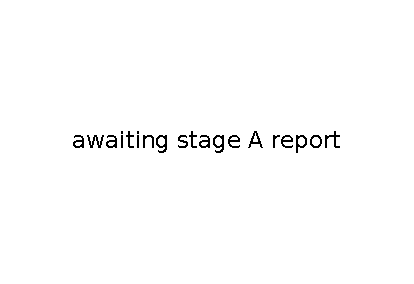
\includegraphics[width=\columnwidth]{figures/fig_h3.pdf}
\caption{Stage A matched pairs. The horizontal axis is the locked gap in transfer precision and the vertical axis is the gap in endpoint held-out oracle accuracy. Natural pairs are diamonds. Each pair shares one step-0 rate, so $J$ is constant within a pair.}
\label{fig:h3}
\end{figure}

The same pairs are scored by baselines that do not use the screen, and by the structure label that the theory assigns without a statistic: $-1$ for a shared-behaviour rule and $0$ otherwise.
Table~\ref{tab:baselines} reports each baseline's correlation with the accuracy gap and the gap $\rho(\tau) - \rho(b)$.
The class baseline correlates at $\HThreeClassRho{}$, and $\rho(\tau) - \rho(\mathrm{class})$ is $\HThreeClassGap{}$.
Inside the stratum of shared and natural pairs, where the structure label assigns no direction, the correlation is $\HThreeSharedRho{}$ (permutation $p = \HThreeSharedP{}$, 5th percentile $\HThreeSharedQFive{}$, $n = \HThreeSharedN{}$).
The audit that produces $J$, the precisions, the cosine, the probe, the Egashira product, and the screen is shared by every arm in the cell.
The step-25 baseline is one short training run per arm.
% AFTER-RESULTS: (class gap is positive and H3 holds) The screen orders pairs that a shared-versus-other label does not separate.
% AFTER-RESULTS: (class gap is not positive) The structure label accounts for as much of the ranking as the screen on this sample.
% AFTER-RESULTS: (shared stratum holds) The ordering remains inside the shared and natural pairs.
% AFTER-RESULTS: (shared stratum does not hold) The ordering does not remain once the sample is restricted to shared and natural pairs.

\begin{table*}[t]
\caption{Baselines for the stage A accuracy gaps. $\rho$ is the baseline's Spearman correlation. The last column is where the number comes from. The note under the table is the break-even count of verifiers.}
\label{tab:baselines}
\centering
\small
\setlength{\tabcolsep}{4pt}
\begin{tabular}{lrrp{0.28\textwidth}}
\toprule
Baseline & $\rho$ & $\rho(\tau)-\rho(b)$ & Cost \\
\midrule
step-0 Youden J & \pending & \pending & shared audit \\
mean precision & \pending & \pending & shared audit \\
modal precision & \pending & \pending & shared audit \\
$\cos(g_V, g_O)$ & \pending & \pending & shared audit \\
held-out probe AUC & \pending & \pending & shared audit \\
step-25 accuracy & \pending & \pending & one 25-step run per verifier \\
Egashira et al.\ $f \times C$ & \pending & \pending & shared audit \\
shared-behaviour label & \pending & \pending & rule label, no training \\
\bottomrule
\end{tabular}

The audit, with its features, is paid once per cell and serves every verifier; a step-25 run is one short training job per verifier. From recorded wall time, one audit costs as much as \BreakEvenMeasured{} step-25 runs. No projected ratio is quoted: the plan does not price the audit's gradient pass.

\end{table*}

\subsection{Same class, opposite direction}
\label{sec:h10}

H10 holds the structure class fixed.
For each pair $(a, b)$ the estimate is the equal-weight mean over conclusive E1 cells of $\mathrm{sign}(\Delta\tau)\,(\mathrm{acc}_a - \mathrm{acc}_b)$, with the locked $\Delta\tau = \tau_{\mathrm{pool}}(a) - \tau_{\mathrm{pool}}(b)$.
The pairs are $(\texttt{fp\_trigger\_enriched}, \texttt{fp\_trigger})$ and $(\texttt{fn\_behavior\_depleted}, \texttt{fn\_behavior})$.
The aligned gaps are $\HTenTrigger{}$ (one-sided $p = \HTenTriggerP{}$) and $\HTenFn{}$ (one-sided $p = \HTenFnP{}$), with Holm correction across the two pairs and a minimum of three cells.
A negative $\Delta\tau$ flips the accuracy gap before the average, so a rule that merely says shared errors are bad cannot pass.
Only the direction the screen reads can.
% AFTER-RESULTS: (H10 holds) The screen separates two shared phrase rules that have the same rate and the same class.
% AFTER-RESULTS: (H10 does not hold) The screen does not separate the same-class phrase pairs on the preregistered test.

\subsection{Natural verifiers and patching}
\label{sec:h7}

H7 tests whether a natural verifier differs from resampled noise at its own rate.
The family has five pairs: two in math, and one each in code, instruction following, and judged question answering.
The number of those pairs whose interval excludes zero is $\HSevenNDiff{}$.
For every pair that differs, the sign of the contrast is compared with the sign of the locked transfer-precision gap.
Figure~\ref{fig:natural} plots each natural verifier's step-0 error rate, $\mathrm{FPR} + \mathrm{FNR} = 1 - J$, against that locked gap and against the endpoint accuracy gap.
H8 is the patch comparison on the domains where the two selections differ.
The equal-weight mean of screen patch minus error-count patch is $\HEightPoint{}$ (one-sided $p = \HEightP{}$, $n = \HEightN{}$ domains).
% AFTER-RESULTS: (H7 holds) At least one natural verifier separates from rate-matched noise.
% AFTER-RESULTS: (H7 does not hold) The natural verifiers do not separate from rate-matched noise on the preregistered test.
% AFTER-RESULTS: (H8 holds) Choosing the two categories by the screen beats choosing them by the error count.
% AFTER-RESULTS: (H8 does not hold) The screen's patch does not beat the error-count patch.

\begin{figure*}[t]
\centering
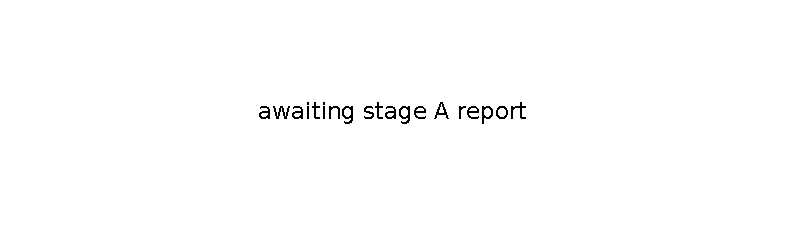
\includegraphics[width=\textwidth,height=1.55in,keepaspectratio]{figures/fig_natural.pdf}
\caption{Natural verifiers in stage A. Each point is one natural verifier. The horizontal axis is its step-0 error rate, $\mathrm{FPR} + \mathrm{FNR} = 1 - J$. The vertical axes are the locked transfer-precision gap and the endpoint accuracy gap, both as natural minus its resampled control. If rate decided fate, every point would sit at zero on both vertical axes.}
\label{fig:natural}
\end{figure*}

\subsection{How many oracle labels}
\label{sec:h9}

H9 recomputes the stage A correlation from the stored draws of $\tau_{\mathrm{pool}}$ at 32, 64, 128, and 192 labels.
Draws are not imputed.
The median correlations are $\HNineMedThirtyTwo{}$, $\HNineMedSixtyFour{}$, $\HNineMedOneTwoEight{}$, and $\HNineMedOneNineTwo{}$.
The 5th percentiles are $\HNineQThirtyTwo{}$, $\HNineQSixtyFour{}$, $\HNineQOneTwoEight{}$, and $\HNineQOneNineTwo{}$.
The fractions of draws with positive correlation are $\HNinePosThirtyTwo{}$, $\HNinePosSixtyFour{}$, $\HNinePosOneTwoEight{}$, and $\HNinePosOneNineTwo{}$.
Figure~\ref{fig:h9} plots the medians.
H9 is secondary.
% AFTER-RESULTS: (the median rises toward 192) Extra labels past the smallest budget move the screen.
% AFTER-RESULTS: (the median is flat) The smaller budgets already match the 192-label screen on this sample.

\begin{figure}[t]
\centering
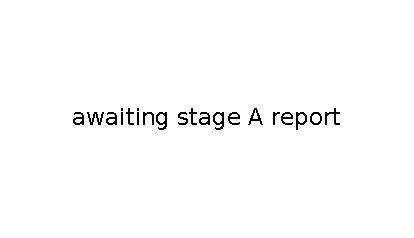
\includegraphics[width=\columnwidth,height=1.55in,keepaspectratio]{figures/fig_h9.pdf}
\caption{Oracle-label budget for the stage A screen. The curve is the median correlation of the stored $\tau_{\mathrm{pool}}$ draws with the endpoint accuracy gap, at each number of oracle labels.}
\label{fig:h9}
\end{figure}

\section{Replication at scale and across families: stage B}
\label{sec:replication}

Stage B is computed once, on its own pairs, after its own runs.
Stage A's pairs do not enter the test.
H3-replication is the same three gates as H3: a within-cell permutation $p$-value below 0.05, a bootstrap 5th percentile above 0, and at least 20 pairs.
The correlation on stage B is $\HThreeRepRho{}$ (permutation $p = \HThreeRepP{}$, 5th percentile $\HThreeRepQFive{}$, $n = \HThreeRepN{}$).
% AFTER-RESULTS: (H3-replication holds) The screen orders pairs on models and families that stage A did not use to choose the test.
% AFTER-RESULTS: (H3-replication does not hold) The screen's ordering does not replicate on the stage B pairs.

The secondary union, which is computed only when both stages are complete, has correlation $\HThreeAllRho{}$ (permutation $p = \HThreeAllP{}$, 5th percentile $\HThreeAllQFive{}$, $n = \HThreeAllN{}$).
Scale slopes are ordinary least squares of each kit contrast on $\log_{10}$ of the model specification's parameter count, with a cell-level bootstrap interval.
They are secondary, and they are empty until the ladder is complete.
Appendix~\ref{app:cells} prints the slope table.
% AFTER-RESULTS: (union holds) Pooling the stages does not remove the ordering.
% AFTER-RESULTS: (union does not hold) The pooled correlation does not clear the same three gates.
% AFTER-RESULTS: (slopes are flat) The kit gaps do not show a monotone scale trend on this ladder.
% AFTER-RESULTS: (slopes are not flat) Read each slope's interval before describing a scale trend. The intervals are in the appendix table.

\section{Related work}
\label{sec:related}

\paragraph{Pattern and rate.}
\citet{egashira2026delay} plant systematic verifier errors and conclude that the outcome is not determined by the overall error rate.
Their arms are not calibrated to one rate.
\citet{rad2026rate} analyse class-conditional noise as a replicator flow and find that, when $J > 0$, noise primarily rescales convergence time.
The study's synthetic channel has $J = 0.55$, so that result predicts that the resampled arms still learn.
It does not predict that a resampled arm matches a clean verifier, and this paper does not make that prediction.
\citet{plesner2026noise} find symmetric noise up to 15 percent close to clean training and ask for fixed noise with the two rates varied separately.
\citet{mitsuhashi2026scaling} find that an accuracy gap under controlled noise persists under compute scaling.
\citet{zhu2026incorrect} report that incorrect annotations remain costly after a contamination check, against earlier results in which a large flip rate still learned \citep{lv2025flips}.
\citet{shao2025spurious} show that random rewards can raise accuracy through clipping; the reported random arm in the math cell is that reference point and is outside every hypothesis.

\paragraph{Natural errors and audits.}
\citet{zhang2026leaky} compare original and hardened tests on MBPP and find that rewarded false-positive mass tracks a static leakiness audit.
The comparison has no rate-matched random arm, and the audit predicts false-positive mass rather than accuracy.
One reading, which is an interpretation and not that paper's claim, is that those natural false positives are the prompt-specific case of Theorem~\ref{thm:transfer}.
H7 is the rate-matched test of natural verifiers.
\citet{xin2026audit} audit math verifiers by category, and the two natural math verifiers here are the relative tolerance and the strip-string match that audit discusses.
\citet{xin2026correlation} measure within-group error correlation.
A prompt-specific rule is correlated within a group and is still predicted to stay local, and the prompt-centred statistics here remove the shared prompt-difficulty component.
\citet{ray2026fuzz} and \citet{zhou2026language} document verifier failures and do not forecast a training outcome.

\paragraph{Judges, probes, and corrections.}
\citet{zhao2025token} show master-key false positives against model judges.
\citet{huang2025hacking} find model-based math verifiers susceptible to reward hacking during reinforcement learning.
The judged question-answering domain trains against a real judge \citep{ma2025reasoner}, with the robust judge of \citet{zhao2025token} as a reported second natural verifier, outside the hypotheses.
A master key is a shared surface feature, the same role as the phrase trigger.
Probes fit during training can forecast hacking before the visible rate is high \citep{beigi2026probes,wang2026grift,bergen2026means,karmakar2026judge}.
Those methods act during or after training.
The screen here is computed once, at step 0, and then locked.
A correction that uses only the known rates is identical for an arm and its rate-matched control, so it cannot explain a difference between them \citep{cai2025correct,mansouri2025correct}.
With group-standardised advantages, an affine reward correction also leaves the GRPO update unchanged.

\paragraph{Geometry, features, and the training rule.}
Lemma~\ref{lem:tilt} quotes the exponential-tilt geometry of \citet{mroueh2025tilt} and \citet{dorner2025tilt} and is not claimed as new.
Proposition~\ref{prop:mode} is the Euclidean softmax flow.
Theorem~\ref{thm:transfer} is the part about fixed errors and held-out prompts.
\citet{stroebl2024limits} study imperfect verifiers at inference, as best-of-$n$ selection; the object here is training.
\citet{xia2024less} and \citet{park2023trak} use random projections of gradients for data selection and influence.
At LoRA initialisation the trainable step-0 feature is already such a projection \citep{hu2021lora}, and CountSketch keeps the inner product unbiased \citep{charikar2002frequent}.
Work on updates that concentrate in a small part of the network is the regime in which one step-0 direction can summarise what training reinforces \citep{subnetworks2025rl,razor2025rl}.
Reward hacks can generalise past the task that taught them \citep{macdiarmid2025hacks,taylor2025harmless,daniels2026preference}; the screen asks the narrower question of which fixed errors reach held-out prompts of the same task.

\section{Limitations}
\label{sec:limits}

The screen is a first-order statistic at the base policy.
The knife-edge world is the documented case in which transfer precision is high and the shared flow still collapses (Appendix~\ref{app:proofs}).
A run whose held-out accuracy rises at least 0.05 above step 0 and later falls at least 0.10 below its running peak is labelled knife-edge.
The label does not change a hypothesis.

The features and the trained models are LoRA adapters that share one draw of $A$.
The exploratory full-parameter run (X5) keeps the LoRA screen as its forecast, so it checks the fate and not a full-parameter feature.
Qwen3 is trained in non-thinking mode, the confirmatory horizon is 300 steps, and X7 extends three arms to 600 steps as an exploratory check.

The synthetic arms are planted; H7 answers with verifiers a practitioner would ship, and H10 with two planted rules of the same rate and structure class.
Judge-based oracles, in instruction following and in the adjudication of natural errors, are checked against a second annotator or a second model, and those checks do not change a verdict.

Compute is projected until pilot P5 measures token rates (Appendix~\ref{app:compute}).
A budget cut removes stage B cells in a fixed order, 32B math, the two E3 code cells, 14B code, then 8B question answering, and cannot remove a stage A cell.

\section{Conclusion}
\label{sec:conclusion}

A verifier error is a direction in the step-0 update, and a rate does not determine that direction.
Resampled noise rescales the oracle update, a shared behaviour can transfer, and a prompt-specific error stays local.
Sections~\ref{sec:results} and~\ref{sec:replication} test whether the locked screen, which reads that direction from the outputs it favours, orders held-out accuracy at one rate and inside one structure class.


\section*{Impact Statement}
\label{sec:impact}
This paper measures how a faulty verifier steers reinforcement learning.
A screen that ranks verifiers before training can be used to reject a leaky reward, and the same screen can be used to search for a leak that transfers.
The matched-rate arms are synthetic rules on public reasoning, code, and instruction benchmarks.
They are not an attack on a deployed system, and the paper does not provide a procedure for planting a verifier error in someone else's training run.
Judge-based rewards can disagree with a rule and with a person.
The study reports those disagreements and does not treat a model judge as a substitute for the oracle outside the preregistered checks.
The broader practice this work argues against is shipping a verifier because its error rate looks moderate.
Whether the screen improves that practice is the preregistered result, not a claim this statement settles.


\bibliographystyle{icml2026}
\bibliography{refs}

\appendix
\section{Proofs}
\label{app:proofs}

The statements below are the ones the theory note records.
Assumptions are stated with each result.
Checks are the committed pilot P0 values, printed by the macros and by Tables~\ref{tab:p0fates} and~\ref{tab:p0checks}.
The repository checks the finite-world case of the tilt geometry and does not re-prove \citet{mroueh2025tilt} or \citet{dorner2025tilt}.

\begin{lemma}[Tilt invariance]
\label{lem:tilt}
An update $\pi_t(y \mid x) \propto \pi_0(y \mid x) \exp(g_t(x, V(x,y)))$ preserves $\pi_t(\cdot \mid V = v, x) = \pi_0(\cdot \mid V = v, x)$ on every prompt with $\pi_0(V = v \mid x) > 0$.
\end{lemma}

\begin{proof}
The output space is finite, so the normaliser is a sum.
The multiplier depends on the output only through $V(x,y)$, the base $\pi_0$ is held fixed, and $V$ does not change with $t$.
On the level set $\{y : V(x,y) = v\}$ the factor $\exp(g_t(x,v))$ does not depend on $y$, so it cancels in the conditional.
Specialise to $g_t(x,v) = t v$.
For binary $V$ and a prompt that puts positive mass on both values, let $\alpha_t(x) = \pi_t(V = 1 \mid x)$, $\mathrm{Prec}_0(x) = \mathbb{E}_{\pi_0}[O \mid V = 1, x]$, and $\mathrm{FOR}_0(x) = \mathbb{E}_{\pi_0}[O \mid V = 0, x]$.
Invariance gives
\[
\mathbb{E}_{\pi_t}[O \mid x] = \alpha_t(x)\,\mathrm{Prec}_0(x) + (1 - \alpha_t(x))\,\mathrm{FOR}_0(x).
\]
As $t \to +\infty$, accuracy tends to mean precision.
As $t \to -\infty$, accuracy tends to the false-omission rate.
If a prompt has no mass on one verdict, that endpoint is undefined and the forecast substitutes the prompt's base accuracy.
The committed maximum absolute conditional error is $\PZeroTiltErr{}$.
The $t \to +\infty$ endpoint matches prompt-mean precision to $\PZeroPrecGap{}$.
\end{proof}

\begin{proposition}[Euclidean policy gradient is mode-seeking]
\label{prop:mode}
Under a tabular softmax and the objective $\mathbb{E}_\pi[V] - \beta\,\mathrm{KL}(\pi \| \pi_0)$, Euclidean gradient ascent on the logits is mode-seeking inside a level set of $V$.
For $\beta = 0$ and two outputs with the same verifier value $v$,
\[
\frac{d}{dt} \log \frac{\pi_y}{\pi_{y'}} = \eta \, a_t \, (\pi_y - \pi_{y'}), \qquad a_t = v - \mathbb{E}_\pi[V].
\]
The $\beta = 0$ limit, when the mode is unique, is modal precision.
For every $\beta > 0$ the unique equilibrium is $\pi \propto \pi_0 \exp(V / \beta)$.
\end{proposition}

\begin{proof}
The gradient is Euclidean in the logits: $\partial \mathbb{E}_\pi[V] / \partial z_y = \pi_y (V_y - \mathbb{E}_\pi[V])$.
With $\beta = 0$, $\dot z_y = \eta \, \pi_y (V_y - \mathbb{E}_\pi[V])$.
If $V_y = V_{y'} = v$, the pairwise identity follows because log-odds are logit differences.
On the accepted set, $a_t = \pi(V = 0) \ge 0$, and $a_t > 0$ while any rejected mass remains, so the $\pi_0$-ordering inside $\{V = 1\}$ is preserved and strict gaps grow.
Exact ties have derivative zero and stay ties, so the terminal accuracy averages the tied argmax with $\pi_0$ weights.
The objective is strictly concave in $\pi$ for $\beta > 0$.
Stationarity under $\sum_y \pi_y = 1$ gives $V(y) - \beta \log(\pi(y)/\pi_0(y)) = \lambda$, hence the finite tilt.
For $J > 0$ that tilt sits strictly between base accuracy and mean precision.
The $\beta = 0$ mode is where the unconstrained flow ends after it has left the exponential family.
It is not stationary for any $\beta > 0$.
A shared linear head cannot realise an arbitrary per-prompt tilt.
The committed tabular gap at $\beta = 0$ is $\PZeroModalGap{}$, and the committed gap of the positive-penalty flows is $\PZeroBetaGap{}$.
At $\beta = 0.5$ the theory note records equilibrium accuracy $0.3701$, mean precision $0.5028$, and modal precision $0.3000$.
\end{proof}

\begin{theorem}[Which errors move held-out prompts]
\label{thm:transfer}
Because $V = O - \mathrm{FN} + \mathrm{FP}$ on every sample, $g_V = g_O - g_{\mathrm{FN}} + g_{\mathrm{FP}}$.
Class-conditional noise with rates $\rho_0 = \mathbb{P}(V = 1 \mid O = 0)$ and $\rho_1 = \mathbb{P}(V = 0 \mid O = 1)$, redrawn independently of $\phi$ given $O$, satisfies $\mathbb{E}[g_V] = J g_O$ with $J = 1 - \rho_0 - \rho_1$.
A held-out prompt $x'$ moves only through $\theta$, and to first order $s(y) = \langle \phi(x', y), g_V \rangle$ is the growth rate of $\log \pi(y \mid x')$.
\end{theorem}

\begin{proof}
Covariance is linear in the reward.
Substitute $\mathrm{FN} = O(1-V)$ and $\mathrm{FP} = (1-O)V$:
\[
O - O(1-V) + (1-O)V = V.
\]
Taking the covariance and then the expectation over prompts yields the split.
The committed decomposition error is $\PZeroDecompErr{}$.
Conditioning gives $\mathbb{E}[V \mid O] = \rho_0 + J O$.
Independence of the coins and $\phi$ given $O$ pulls the expectation inside the covariance, the constant $\rho_0$ drops out, and $\mathbb{E}[g_V] = J g_O$.
The committed cosine between the Monte Carlo mean and $J g_O$ is $\PZeroCosine{}$, and the least-squares multiplier differs from 1 by $\PZeroScaleGap{}$.
The first-order velocity freezes $g_V$ at $\pi_0$.
Prompt-specific logits are not applied on held-out prompts, so $x'$ moves only through the shared inner product.

A fixed false-positive bit that is a function of a shared behaviour, with that behaviour a coordinate of $\phi$ on held-out prompts, gives $g_{\mathrm{FP}}$ a component along the coordinate.
The phrase trigger is this case.
A bit that depends on the prompt and is independent of the shared coordinates has prompt-averaged covariance zero.
In the toy worlds the shared exploit and its twin share $J$ and do not share the held-out fate: the committed gaps are $\PZeroHandGap{}$ and $\PZeroRfGap{}$, and the resampled arm stays within $\PZeroHandClose{}$ and $\PZeroRfClose{}$ of the twin.
\end{proof}

\subsection{Transfer precision, advantages, and the sketch}

Exact $\tau$ is the $\pi_0$-weighted oracle accuracy of the held-out outputs that maximise $s = \phi g_V$, with ties averaged.
On the 28-cell grid used to choose $q = 1/32$, its Spearman correlation with trained held-out accuracy is $\PZeroExactRho{}$, against $\PZeroJRho{}$ for step-0 $J$.
The cell it misses is \texttt{rf05} / \texttt{fnC}: exact $\tau = \PZeroFnCTau{}$, observed accuracy $\PZeroFnCObs{}$, and $\tau_{\mathrm{pool}} = \PZeroFnCPool{}$.
That is a fact about this grid.

With $n$ audit samples per prompt, a soft tilt of strength $\kappa$ has the self-normalised estimator $\hat\tau(\kappa) = \mathbb{E}_{x'} (\sum_i O_i e^{\kappa s_i}) / (\sum_i e^{\kappa s_i})$.
The hard limit is at most the fraction of held-out prompts with a correct sample.
Dividing by the same hard limit in the oracle direction cancels that ceiling and does not cancel inflation from missing the favoured output.
The committed Spearman correlation of that ratio is $\PZeroTauRelRho{}$, recorded and not used as a gate.

$\tau_{\mathrm{pool}}(q)$ prompt-centres the velocities, pools them, and takes the oracle accuracy of the top fraction $q$, with $k = \max(1, \mathrm{round}(q N))$ and boundary ties shared equally.
$q = 1/32$ was fixed before any language-model run.
The committed Spearman correlation is $\PZeroTauPoolRho{}$, the within-band fraction is $\PZeroWithin{}$, and the mean split-half cosine of $g_V$ is $\PZeroReliability{}$.
Sum features under a sequence-mean loss divide the train rows that form $g$ by completion length.
Held-out velocities stay undivided, so $s$ is the change in sequence log-probability.
The group-standardised direction is stored and is not the preregistered statistic.

Inside a group of size $G$, with $\mathbb{E}[V_i \mid O_i] = \rho_0 + J O_i$,
\[
\mathbb{E}[A_1 \mid O_1] = \Bigl(1 - \frac{1}{G}\Bigr) J (O_1 - p).
\]
The false-positive rate cancels.
Dividing by a positive group standard deviation does not change the sign of a nonzero advantage inside the group.
Across prompts the scales differ, so the averaged direction can move.
The committed maximum absolute $z$ for the identity is $\PZeroGroupZ{}$.

At LoRA initialisation, $B = 0$, the adapter output is zero, and $\partial L / \partial A = 0$.
The $B$ gradient is the full linear-map gradient with the layer input replaced by $Ax$.
For a CountSketch $S$ of dimension $D$ with the same buckets and signs on both arguments, $\mathbb{E}[\langle Sa, Sb \rangle] = \langle a, b \rangle$, and
\[
\mathrm{Var}(\langle Sa, Sb \rangle) \le \frac{\lVert a \rVert^2 \lVert b \rVert^2 + \langle a, b \rangle^2}{D}.
\]
The cross term has mean zero, and a pair of summands in its second moment survives only when the index pairs coincide, which brings the factor $1/D$.

\subsection{The knife-edge}

$\tau$ uses $g_V$ at $\pi_0$.
The counterexample is outside the 28-cell grid.
Four atoms share a base mass on every prompt: a correct accepted atom on the skill coordinate with mass $0.15$; an incorrect accepted atom on an exploit coordinate of amplitude $1.10$ with mass $0.12$; a rejected atom at $0.99$ of the skill direction with mass $0.003$; and a rejected noise atom with mass $0.727$.
Mean precision is $0.15 / 0.27 = 0.5556$.
The false-positive rate is $0.12 / 0.85$, the false-negative rate is $0$, and $J = 0.8588$, matching $\PZeroKnifeJ{}$ from the committed rows.
The committed transfer precisions run from $\PZeroKnifeTauMin{}$ to $\PZeroKnifeTauMax{}$.
The theory note records an initial slope of held-out accuracy of $0.0119$ and peaks from $0.5465$ to $0.5768$.
Along the shared flow the skill coordinate also raises the rejected impure atom, the skill covariance with $V$ falls, and the exploit coordinate does not pick up that penalty.
Mean terminal held-out accuracy is $\PZeroKnifeTerminal{}$.
The one-percent detune, plus feature noise of scale $0.008$, makes the top-velocity output unique.
A failure of this world to rise and then collapse would mean the counterexample had not been reproduced.

\section{Preregistration, stages, and deviations}
\label{app:prereg}

The confirmatory families, margins, bootstrap, and permutation counts are those in Section~\ref{sec:study}.
Stage A is discovery: \texttt{e1-chain\_sum-qwen3-1.7b}, \texttt{e1-math-qwen3-1.7b}, \texttt{e1-code-qwen3-1.7b}, \texttt{e1-ifeval-qwen3-1.7b}, \texttt{e1-qa-qwen3-1.7b}, and the five E2 cells at Qwen3-4B.
Stage B is replication: Qwen3-8B on math, code, and question answering; Qwen3-14B on math and code; Qwen3-32B on math; OLMo-3-7B-SFT on math and code; and Llama-3.1-8B-Instruct on math and code.
Each stage is analysed once, when it is complete.
The deviation log is whatever the report contains.

The preregistration's deviation log is empty. The report lists none.


\section{Domains, pools, and oracles}
\label{app:domains}

\begin{table*}[t]
\caption{Domains. The natural verifier is what a practitioner would ship. It is not calibrated to the synthetic rate.}
\label{tab:domains}
\centering
\small
\begin{tabular}{p{0.16\textwidth}p{0.26\textwidth}p{0.22\textwidth}p{0.22\textwidth}}
\toprule
Domain & Source & Oracle & Natural verifier \\
\midrule
chain sum & Reasoning Gym decimal chain sum & exact decimal equality & exact string match, audited \\
math & Big-Math-RL-Verified, decontaminated & symbolic equivalence & lenient cascade; strict string match \\
code & TACO, Python & every hidden test passes & public examples in the statement \\
instruction following & IFEval and IFBench constraints & checkers and a content judge & checkers alone \\
qa & WebInstruct-verified & strict rule & 1.5B model judge \\
\bottomrule
\end{tabular}

\end{table*}

Every domain uses 1,024 train prompts and 384 held-out prompts, plus a development pool for the pilots, disjoint after deduplication.
Splits are a salted hash of the question, fixed before sampling.
Difficulty is a bucket chosen by pilot P2, not a question dropped because of how the study model answered it.

Chain sum is Reasoning Gym \texttt{decimal\_chain\_sum} in the configuration of \citet{egashira2026delay}: 3 to 6 terms, 3 to 6 digits, and 3 to 6 decimal places.
The oracle is exact decimal equality of the last boxed answer, at a 1,024-token budget.
The string-match verifier is audited and not trained.

Math is Big-Math-RL-Verified with proofs and multiple choice removed, and with statements that match MATH-500, the GSM8K test set, or AIME 1983 to 2024 removed \citep{albalak2025bigmath}.
Buckets are the dataset's Llama-8B solve-rate bands from $[0, 0.2)$ through $[0.6, 0.8)$.
The oracle is symbolic equivalence of the last box, with floats rounded to 6 decimal places and no relative tolerance, on a 5-second CPU limit.
A timeout is incorrect.
The lenient natural verifier accepts the last box or the last number at relative tolerance $10^{-4}$.
The strict one is strip-string exact match.
The token budget is 1,536.

Code is TACO, Python only, with at least five hidden tests and a public example in the statement \citep{li2023taco}.
Easy is the dataset's easy bucket.
Medium is the medium bucket together with medium-hard, because medium alone is 740 train and 250 held-out problems, short of the pools.
There is no backup source.
The oracle passes a fixed hashed subset of at most 32 hidden tests, at 2 seconds and 512 MB each.
The process that runs a submission never holds an expected output.
A guard installed in that process refuses file, process, and network access outside its working directory, and on Linux it is preceded by Landlock when the kernel provides it.
Refused operations are counted per sample.
The natural verifier runs the public examples in the statement.
An example whose input is also a hidden test is scored against that test's expected output.
The token budget is 1,024.

Instruction following uses AllenAI's multi-constraint data with IFEval and IFBench checkers \citep{pyatkin2025ifbench,lambert2024tulu}.
Buckets are 2 to 3 constraints and 4 to 5 constraints.
The oracle requires every checker and a frozen Qwen3-14B content judge in non-thinking mode at temperature 0.
The natural verifier is the checkers alone, so its false-negative rate is 0 by construction.
The token budget is 768.
Agreement with \texttt{gpt-4.1} is computed on 500 held-out evaluation samples after training and does not change a verdict.

Question answering is WebInstruct-verified, restricted to answers with a canonical form \citep{ma2025reasoner}.
The oracle is symbolic equivalence or normalised exact match, with no tolerance.
The natural verifier is the 1.5B general verifier.
The token budget is 1,024.
Before the E1 lock, one annotator labels about 200 held-out audit samples on which the rule, Qwen3-32B, and an API model disagree.
Pilot P6 adjudicates 100 step-0 false positives of each natural verifier on the development pool.
None of these checks changes a verdict.

Backups exist only for the pilot screens: DeepScaleR without AIME for math, and a second instruction-following source.
Chain sum, code, and question answering have none.
A source that fails to load stops the audit.

\section{Arms and calibration}
\label{app:arms}

Targets, phrase rules, and the decoy are fixed in the arms files before sampling.
The preference sign is the within-prompt association of the phrase with correctness, so a phrase that only marks a kind of prompt does not count as a behaviour.
Candidates are proposed on seven eighths of the train prompts.
The sign is checked on prompts with $u_{01}(\texttt{phrase\_validation}, \mathrm{pid}) < 1/8$.
The rate tolerance is 0.02 on the full train pool.
\texttt{fp\_trigger} passes the sign check if the validation association is at most 0 or its 90 percent prompt-bootstrap interval covers 0.
\texttt{fp\_trigger\_enriched} and \texttt{fn\_behavior} pass if the validation association is positive.
\texttt{fn\_behavior\_depleted} passes if it is negative.
A phrase arm with no candidate inside the tolerance, or a failed sign check, is withdrawn.

The chain-sum decoy's lower edge is the fitted tolerance of \texttt{fp\_tolerance}.
Its upper edge is the smallest observed error whose pooled false-positive rate is closest to 0.15.
The two arms accept disjoint sets of wrong answers.
A difference between their fates is not explained by the rate or by answer formatting.
The decoy contrast is reported beside H1 and is outside the Holm family.

Patch categories are cheap predicates fixed in the task module before sampling.
Both patch arms fix $k = 2$ categories.
The selection runs after the features and before the lock.
Natural verifiers are never withdrawn for their rate.
A resampled control uses the matched arm's channel rates and the support named in the kit table.

\section{Training and hardware}
\label{app:train}

The audit generator, the gradient features, and the training policy use the same checkpoint, chat template, token budget, and temperature.
LoRA $A$ is saved by the audit and loaded by every seed, at rank 16, $\alpha = 32$, on all seven projections of every layer, with \texttt{lora\_seed} $= 0$.
Model weights are bfloat16.
Sketched gradients accumulate in float32.
CountSketch dimension is 8,192 at sketch seed 0.
Rollouts use temperature 1 and top-$p$ $1$, with no per-request seed, so seeds sample that variation rather than a bit-identical run.
The learning rate warms up linearly for 10 steps.
There is no importance-sampling correction and one update per batch.
Evaluation uses 4 samples on each of the 384 held-out prompts and 128 train prompts.
Every trained arm also runs seed 99 for 25 steps.
That run is the step-25 baseline and is not confirmatory.

Qwen3 checkpoints run with thinking disabled in sampling, features, training, and evaluation \citep{qwen2025qwen3}.
OLMo-3 uses \texttt{allenai/Olmo-3-7B-Instruct-SFT}, the supervised checkpoint, at learning rate $1 \times 10^{-5}$.
Llama-3.1-8B-Instruct uses its shipped template at the same learning rate.
Versions are pinned in the GPU setup script and copied into every lock.
A cell's audit, training, and early baselines run on that cell's hardware class.
Training refuses another class.
Pooled analyses use within-cell differences only.

For each E1 domain, if the sample standard deviation of the two pilot oracle seeds on the development pool exceeds 0.03, that cell's H1 and H2 arms also run seeds 3 and 4.
The seed list is written into the cell configuration before its audit.

\section{Per-cell and secondary tables}
\label{app:cells}

\begin{table*}[t]
\caption{Confirmatory cells. Oracle gain and the conclusive bit stay pending until the stage report publishes them.}
\label{tab:cells}
\centering
\small
\setlength{\tabcolsep}{3pt}
\begin{tabular}{p{0.22\textwidth}cp{0.12\textwidth}p{0.14\textwidth}p{0.16\textwidth}cc}
\toprule
Cell & Stage & Domain & Model & Hardware & Gain & Conclusive \\
\midrule
\texttt{e1-\allowbreak{}chain\_sum-\allowbreak{}qwen3-\allowbreak{}1.7b} & A & chain\_sum & qwen3-\allowbreak{}1.7b & rtx-\allowbreak{}a6000-\allowbreak{}48gb & \pending & \pending \\
\texttt{e1-\allowbreak{}math-\allowbreak{}qwen3-\allowbreak{}1.7b} & A & math & qwen3-\allowbreak{}1.7b & rtx-\allowbreak{}a6000-\allowbreak{}48gb & \pending & \pending \\
\texttt{e1-\allowbreak{}code-\allowbreak{}qwen3-\allowbreak{}1.7b} & A & code & qwen3-\allowbreak{}1.7b & rtx-\allowbreak{}5000-\allowbreak{}ada-\allowbreak{}32gb & \pending & \pending \\
\texttt{e1-\allowbreak{}ifeval-\allowbreak{}qwen3-\allowbreak{}1.7b} & A & ifeval & qwen3-\allowbreak{}1.7b & rtx-\allowbreak{}5000-\allowbreak{}ada-\allowbreak{}32gb & \pending & \pending \\
\texttt{e1-\allowbreak{}qa-\allowbreak{}qwen3-\allowbreak{}1.7b} & A & qa & qwen3-\allowbreak{}1.7b & rtx-\allowbreak{}5000-\allowbreak{}ada-\allowbreak{}32gb & \pending & \pending \\
\texttt{e2-\allowbreak{}chain\_sum-\allowbreak{}qwen3-\allowbreak{}4b} & A & chain\_sum & qwen3-\allowbreak{}4b & a100-\allowbreak{}80gb & \pending & \pending \\
\texttt{e2-\allowbreak{}math-\allowbreak{}qwen3-\allowbreak{}4b} & A & math & qwen3-\allowbreak{}4b & a100-\allowbreak{}80gb & \pending & \pending \\
\texttt{e2-\allowbreak{}code-\allowbreak{}qwen3-\allowbreak{}4b} & A & code & qwen3-\allowbreak{}4b & a100-\allowbreak{}80gb & \pending & \pending \\
\texttt{e2-\allowbreak{}ifeval-\allowbreak{}qwen3-\allowbreak{}4b} & A & ifeval & qwen3-\allowbreak{}4b & a100-\allowbreak{}80gb & \pending & \pending \\
\texttt{e2-\allowbreak{}qa-\allowbreak{}qwen3-\allowbreak{}4b} & A & qa & qwen3-\allowbreak{}4b & a100-\allowbreak{}80gb & \pending & \pending \\
\texttt{e2-\allowbreak{}math-\allowbreak{}qwen3-\allowbreak{}8b} & B & math & qwen3-\allowbreak{}8b & h100-\allowbreak{}80gb & \pending & \pending \\
\texttt{e2-\allowbreak{}code-\allowbreak{}qwen3-\allowbreak{}8b} & B & code & qwen3-\allowbreak{}8b & h100-\allowbreak{}80gb & \pending & \pending \\
\texttt{e2-\allowbreak{}qa-\allowbreak{}qwen3-\allowbreak{}8b} & B & qa & qwen3-\allowbreak{}8b & h100-\allowbreak{}80gb & \pending & \pending \\
\texttt{e2-\allowbreak{}math-\allowbreak{}qwen3-\allowbreak{}14b} & B & math & qwen3-\allowbreak{}14b & h100-\allowbreak{}80gb & \pending & \pending \\
\texttt{e2-\allowbreak{}code-\allowbreak{}qwen3-\allowbreak{}14b} & B & code & qwen3-\allowbreak{}14b & h100-\allowbreak{}80gb & \pending & \pending \\
\texttt{e2-\allowbreak{}math-\allowbreak{}qwen3-\allowbreak{}32b} & B & math & qwen3-\allowbreak{}32b & h100-\allowbreak{}80gb & \pending & \pending \\
\texttt{e3-\allowbreak{}math-\allowbreak{}olmo3-\allowbreak{}7b} & B & math & olmo3-\allowbreak{}7b & h100-\allowbreak{}80gb & \pending & \pending \\
\texttt{e3-\allowbreak{}code-\allowbreak{}olmo3-\allowbreak{}7b} & B & code & olmo3-\allowbreak{}7b & h100-\allowbreak{}80gb & \pending & \pending \\
\texttt{e3-\allowbreak{}math-\allowbreak{}llama3.1-\allowbreak{}8b} & B & math & llama3.1-\allowbreak{}8b & h100-\allowbreak{}80gb & \pending & \pending \\
\texttt{e3-\allowbreak{}code-\allowbreak{}llama3.1-\allowbreak{}8b} & B & code & llama3.1-\allowbreak{}8b & h100-\allowbreak{}80gb & \pending & \pending \\
\bottomrule
\end{tabular}

\end{table*}

\begin{table*}[t]
\caption{Matched pairs from the report. Class is $-1$ for a shared-behaviour rule and $0$ otherwise.}
\label{tab:pairs}
\centering
\small
\setlength{\tabcolsep}{3pt}
No pair rows are in the report yet.

\end{table*}

\begin{table}[t]
\caption{Stage A label budget. Medians are pending until the stored draws are in the report.}
\label{tab:h9}
\centering
\small
\begin{tabular}{lrrr}
\toprule
Labels & Median $\rho$ & 5th pct. & Frac.\ $>0$ \\
\midrule
32 & \pending & \pending & \pending \\
64 & \pending & \pending & \pending \\
128 & \pending & \pending & \pending \\
192 & \pending & \pending & \pending \\
\bottomrule
\end{tabular}

\end{table}

\begin{table}[t]
\caption{Scale slopes of kit contrasts on $\log_{10}$ of the specification's parameter count. Pending until the union secondary is complete.}
\label{tab:scale}
\centering
\small
Scale slopes are pending until stage B is complete.

\end{table}

\section{Compute and cost}
\label{app:compute}

Hours below come from the program planner.
They are projected while any job still uses a placeholder token rate, and measured only after pilot P5 writes a throughput file.
Rented dollars use the planner's H100 price.
Lab classes are priced at zero in that file, so the rented total is mostly stage B.
The preregistration's planning range for rented H100 time is about 8,000 to 10,000 dollars, with about 500 dollars of API budget.
At placeholder token rates stage B projects above that range.
If the plan from measured rates still exceeds it, stage B cells leave in the fixed order of Section~\ref{sec:limits} before any stage B audit, and a cell that leaves is reported as not run.

\begin{table*}[t]
\caption{Projected compute by stage and hardware class.}
\label{tab:compute}
\centering
\small
\begin{tabular}{llrrrr}
\toprule
Stage & Hardware & Jobs & H100 hours & Class hours & USD \\
\midrule
A & a100-\allowbreak{}80gb & 149 & 831.10 & 1511.09 & 0.00 \\
A & rtx-\allowbreak{}5000-\allowbreak{}ada-\allowbreak{}32gb & 203 & 550.28 & 1834.25 & 0.00 \\
A & rtx-\allowbreak{}a6000-\allowbreak{}48gb & 154 & 614.06 & 1754.46 & 0.00 \\
B & h100-\allowbreak{}80gb & 310 & 6826.69 & 6826.69 & 17066.74 \\
exploratory & rtx-\allowbreak{}5000-\allowbreak{}ada-\allowbreak{}32gb & 600 & 14.15 & 47.17 & 0.00 \\
exploratory & rtx-\allowbreak{}a6000-\allowbreak{}48gb & 500 & 189.20 & 540.56 & 0.00 \\
\bottomrule
\end{tabular}

Rates are projected. Placeholder token rates stay projected until pilot P5 writes measured rates. H100-equivalent hours are the planner's \texttt{gpu\_hours}. Class hours divide those by \texttt{speed\_vs\_h100}. Rented dollars use \texttt{usd\_per\_gpu\_hour}. The rented total is \PlanRentedUsd{}.

\end{table*}

The break-even count in Table~\ref{tab:baselines} is recorded audit GPU-hours divided by the mean recorded GPU-hours of one step-25 run, on stage A cells.
It is pending until that timing exists.
A resumed audit records no wall time, so a partial time cannot understate the audit.
The planner prices the audit as generation only and leaves out the gradient pass, so the paper quotes no projected ratio.

\section{Pilot evidence}
\label{app:pilots}

Pilot P0 is the finite-world check of Appendix~\ref{app:proofs}.
Tables~\ref{tab:p0fates} and~\ref{tab:p0checks} are the committed report.

\begin{table}[t]
\caption{Pilot P0 trained held-out accuracy at a matched $J$.}
\label{tab:p0fates}
\centering
\small
\begin{tabular}{llrr}
\toprule
World & Arm & $J$ & Held-out accuracy \\
\midrule
hand\_noisy & fpF & 0.8592 & 0.0006 \\
hand\_noisy & fpI & 0.8592 & 0.9943 \\
hand\_noisy & resampled\_fpF & 0.8592 & 0.9944 \\
rf05 & fpF & 0.8606 & 0.0004 \\
rf05 & fpI & 0.8606 & 0.9917 \\
rf05 & resampled\_fpF & 0.8606 & 0.9916 \\
\bottomrule
\end{tabular}

\end{table}

\begin{table*}[t]
\caption{Pilot P0 checks. Each value is the committed report's number for that check.}
\label{tab:p0checks}
\centering
\small
\setlength{\tabcolsep}{3pt}
\begin{tabular}{p{0.24\textwidth}p{0.42\textwidth}rl}
\toprule
Check & Name & Value & Status \\
\midrule
P0.1 & tilt invariance & \ensuremath{7.22 \times 10^{-16}} & pass \\
P0.2 & pathwise covariance decomposition & \ensuremath{4.86 \times 10^{-17}} & pass \\
P0.3a & resampled noise scales the oracle update & 1.0000 & pass \\
P0.3b & J-\allowbreak{}scaling least-\allowbreak{}squares multiplier & 0.0017 & pass \\
P0.3c & group-\allowbreak{}advantage identity and std-\allowbreak{}norm sign & 1.5915 & pass \\
P0.4a & beta=0 tabular flow reaches modal precision & 0.0012 & pass \\
P0.4b & replicator/tilt terminal is mean precision & \ensuremath{1.11 \times 10^{-16}} & pass \\
P0.4c & beta>0 equilibrium is the finite tilt & 0.0120 & pass \\
P0.5.hand\_noisy.gap & hand\_noisy: resampled held-\allowbreak{}out minus fpF & 0.9938 & pass \\
P0.5.hand\_noisy.close & hand\_noisy: resampled held-\allowbreak{}out vs fpI & \ensuremath{7.55 \times 10^{-5}} & pass \\
P0.5.hand\_noisy.J & hand\_noisy: fpF, fpI and resampled share step-\allowbreak{}0 J & 0.0000 & pass \\
P0.5.rf05.gap & rf05: resampled held-\allowbreak{}out minus fpF & 0.9913 & pass \\
P0.5.rf05.close & rf05: resampled held-\allowbreak{}out vs fpI & \ensuremath{8.02 \times 10^{-5}} & pass \\
P0.5.rf05.J & rf05: fpF, fpI and resampled share step-\allowbreak{}0 J & 0.0000 & pass \\
P0.6.coverage & exact tau within tolerance of held-\allowbreak{}out accuracy & 0.9643 & pass \\
P0.6.spearman & Spearman of exact tau with held-\allowbreak{}out accuracy & 0.8600 & pass \\
P0.6.spearman\_J & exact tau beats step-\allowbreak{}0 J & 0.2248 & pass \\
P0.6.spearman\_prec & exact tau beats step-\allowbreak{}0 precision & 0.3074 & pass \\
P0.7.spearman & 16-\allowbreak{}sample tau\_pool ranks held-\allowbreak{}out accuracy & 0.8617 & pass \\
P0.7.calibration & 16-\allowbreak{}sample tau\_pool within tolerance of held-\allowbreak{}out accuracy & 1.0000 & pass \\
P0.7.tau\_rel & 16-\allowbreak{}sample per-\allowbreak{}prompt tau\_rel ranks held-\allowbreak{}out accuracy & 0.7769 & documented \\
P0.7.reliability & split-\allowbreak{}half reliability of the 16-\allowbreak{}sample velocity & 0.9871 & pass \\
P0.8 & knife-\allowbreak{}edge: tau predicts success, shared flow collapses & 0.0226 & documented \\
\bottomrule
\end{tabular}

\end{table*}

Pilots P1 through P6 are runs before the study.
P1 checks the harness.
P2 chooses each domain's difficulty bucket on the development pool.
P3 checks the estimator, including agreement of bfloat16 features with float32 features.
P4 is a short oracle run in every domain.
P5 is the hardware gate, the seed rule, and the throughput measurement.
P6 adjudicates natural-verifier false positives.
A pilot that fails its preregistered rule removes or replaces a domain before any confirmatory lock.
Those decisions are not confirmatory results, and this appendix does not restate them as hypothesis tests.

\section{Reproducibility}
\label{app:repro}

The anonymous submission includes the code as supplementary material.
The submission checklist records the anonymous archive address.
A cell lock is the SHA-256 of the canonical forecasts, the cell configuration, the environment report, and every artefact the forecasts depend on: pools, step-0 completions, oracle grades, calibration, the arms file, the features, the patch selections, and the LoRA initialisation.
Training refuses to start if any of them has changed, including when the current parser would grade an audited completion differently.

No lock hashes are in the report yet. Each cell's lock is the SHA-256 of the forecasts, the cell configuration, the environment, and every input artefact, written before that cell's first training step.


Generated macros, tables, and figures are produced by \texttt{python -m vfates.paper assets} and are part of the source, so the PDF builds from a clean clone without rerunning the study.
Outcome macros render as pending until the corresponding stage block exists.
The abstract file contains one sentence per confirmatory hypothesis that passed, and no sentence for a hypothesis that did not.


\end{document}
